\section{Differentiation}

  \begin{definition}[Frechet Derivative]
    A function $f: D \subset \mathbb{R}^n \longrightarrow \mathbb{R}^m$ is \textbf{differentiable} at $x \in D$ if there exists a unique linear map $Df_x: \mathbb{R}^n \longrightarrow \mathbb{R}^m$---called the \textbf{total derivative} or \textbf{Frechet derivative}---such that 
    \begin{equation}
      \lim_{h \to 0} \frac{\| f(x + h) - f(x) - Df_x h \|}{\| h \|} = 0 
    \end{equation} 
    If such a map $D f_x$ exists, then it is unique. 
  \end{definition}
  \begin{proof}
    The only claim to prove is uniqueness if defined. 
  \end{proof} 

  The reason we want $D$ to be open is that we require that $x + h$ to also be in $D$ for sufficiently small $h$, and we can guarantee this since an $\epsilon$-ball around $x$ is guaranteed to be in $D$. Just as with the univariate case, the fundamental increment lemma also holds. 

  \begin{lemma}[Fundamental Increment Lemma]
    Suppose the derivative of $f: [a, b] \subset \mathbb{R}^n \to \mathbb{R}$ at $x$ exists. Then, there exists a function $\Phi: \mathbb{R}^n \to \mathbb{R}$ such that 
    \begin{equation}
      f(x + h) = f(x) + Df_x h + \Phi(h) \|h\|
    \end{equation}
    for sufficiently small nonzero $h$, and 
    \begin{equation}
      \lim_{h \to 0} \Phi(h) = 0
    \end{equation}
  \end{lemma}

  Note that when $m = 1$, then $Df_x$ is a linear functional, i.e. a dual vector. A simple way to extract derivatives is to fix all of the input components except for one, and treat $f$ as a single-variable function. This results in---for now---a completely separate notion of a derivative. 

  \begin{definition}[Directional, Partial Derivative]
    The \textbf{directional derivative} of a multivariate function $f: D \subset \mathbb{R}^n \longrightarrow \mathbb{R}$ at a point $\mathbf{a} \in D$ in direction $\mathbf{v} \in \mathbb{R}^n$ is the instantaneous rate of change of $f$ when moving along direction $\mathbf{v}$ at $\mathbf{a}$. Formally, 
    \[\nabla_\mathbf{v} f(\mathbf{a}) \coloneqq \lim_{h \rightarrow 0} \frac{f(\mathbf{a} + h \mathbf{v})}{h}\]
    When computing directional derivatives, it is convenient to normalize the directional vector $\mathbf{v}$ to be unit length so that it coincides with the partial derivatives. We don't technically need to set $||\mathbf{v}|| = 1$, but if we have two vectors $\mathbf{v}$ and a scaled $c \mathbf{v}$, then the directional derivatives will also be scaled ($\nabla_{c \mathbf{v}} f (\mathbf{a}) = c \nabla_{\mathbf{v}} f (\mathbf{a})$), so we will only work with unit directional vectors. Some say that this restriction is undesirable, since it loses the linearity of the function $\mathbf{v} \mapsto \partial_\mathbf{v} f (\mathbf{a})$. 

    If $\mathbf{v}$ is a unit basis vector $\mathbf{e}_i$, then we define this specific instance to be the \textbf{partial derivative} of $f$ with respect to argument $\mathbf{x_i}$. 
    \[\partial_{x_i} f (\mathbf{a}) = \frac{\partial}{\partial x_i} \bigg|_{\mathbf{a}} f \coloneqq \lim_{h \rightarrow 0} \frac{f(\mathbf{a} + h \mathbf{e}_i)}{h} \]
    which can be calculated by differentiating the function w.r.t. $x_i$ and fixing all other variables. The partial derivative looks at the function as it is approaching $\mathbf{a}$ along an axis, while a directional derivative looks at the function as it is approaching from any direction in the domain. 
  \end{definition}

  Therefore, we have sort of three (or two) separate notions of derivatives. A natural question to ask is whether the existence of one derivative implies the existence of another. 

  \begin{theorem}[Existence of Derivatives]
    Let us have a function $f: D \subset \mathbb{R}^n \longrightarrow \mathbb{R}$ and a point $\mathbf{a} \in D$. 
    \begin{enumerate}
      \item If $f$ is differentiable at $\mathbf{a} \in D$, then all of its directional derivatives exist. Furthermore, the total derivative $D f_\mathbf{a}$ applied to the directional unit vector $\mathbf{v}$ is equal to the directional derivative at $\mathbf{a}$ in direction $\mathbf{v}$.
      \begin{equation}
        D f_\mathbf{a} \mathbf{v} = \nabla_\mathbf{v} f (\mathbf{a})
      \end{equation}

      \item If all directional derivatives exist, then the partials exist (since we can just set the directional vectors to be the unit vectors). 
    \end{enumerate}
  \end{theorem} 

  Therefore, we know that differentiability (i.e. existence of the total derivative) is the strongest. If this is the case, then the partial and directional derivatives exist. It turns out that if we know the partial derivative 

  Furthermore, since our vector spaces come with a basis, we can realize $Df_x$ in a matrix form. Furthermore, we can compute it quite easily!

  \begin{definition}[Jacobian]
    Given $f: E \subset \mathbb{R}^n \to \mathbb{R}^m$ differentiable at $x$, the \textbf{Jacobian} of $f$ at $x$ is the matrix realization of the total derivative, denoted $J f_x$. 
  \end{definition} 

  \begin{theorem}[Partial Derivatives as Image of Total Derivative]
    The partial derivative equals the image of the basis vector 
    \begin{equation}
      \frac{\partial f_j}{\partial x_i} = (D f_x e_i)_j
    \end{equation}
  \end{theorem}
  
  \begin{corollary}[Directional Derivatives as Image of Total Derivative]
    The directional derivative equals the image of the direction vector. 
    \begin{equation}
      \nabla_v f(x) = (D f_x v)_j
    \end{equation}
  \end{corollary}
  \begin{proof}
    By linearity. 
  \end{proof}

  \begin{corollary}[Entries of Jacobian are Partials]
    The entries of the Jacobian matrix are precisely the partial derivatives. 
  \end{corollary}
  \begin{proof}
    Immediate result of the previous corollary. 
  \end{proof}

  Analogous to the univariate case, a nice way to visualize the derivative is by looking at the tangent \textit{plane}. In general, we have an \textit{affine hyperplane}. Define this here. Unfortunately, the only types of functions that we can meaningful visualize are those mapping $f: \mathbb{R}^2 \to \mathbb{R}$. 

  \begin{figure}[H]
    \centering 
    % \includegraphics[scale=0.4]{img/}
    \caption{} 
  \end{figure}


  So, to prove that a function $f: \mathbb{R}^n \longrightarrow \mathbb{R}$ is differentiable at $\mathbf{a}$, and if so, what its total derivative is, there are essentially two steps. 
  \begin{enumerate}
    \item We find a candidate for $M$ by evaluating the partials. 
    \[M = \begin{pmatrix} \partial_{x_1} f(\mathbf{a}) & \partial_{x_2} f(\mathbf{a}) & \ldots & \partial_{x_n} f(\mathbf{a}) \end{pmatrix}\]
    \item We check to see if the limit is true. 
    \[\lim_{\mathbf{h} \rightarrow \mathbf{0}} \frac{f(\mathbf{a} + \mathbf{h}) - f(\mathbf{a}) - M \mathbf{h}}{||\mathbf{h}||} = 0\]
    If it is, then $D f_\mathbf{a} = M$, and the "tangent plane" of $f$ at $\mathbf{a}$ is defined by the equation 
    \[y = f(\mathbf{a}) + M \mathbf{h}\]
  \end{enumerate}

  \begin{example}[Computing Total Derivative]
    The function $f(x_1, x_2) = x_1^2 + x_2^2$ is differentiable at $(1, 1)$. We let $M = \big(\partial_{x_1} f(1, 1), \partial_{x_2} f(1, 1) \big) = \big(2, 2\big)$ and see that 
    \begin{align*}
      \lim_{\mathbf{h} \rightarrow \mathbf{0}} \frac{f(\mathbf{a} + \mathbf{h}) - f(\mathbf{a}) - M \mathbf{h}}{||\mathbf{h}||} & = \lim_{\mathbf{h} \rightarrow \mathbf{0}} \frac{f(1 + h_1, 1 + h_2) - f(1, 1) - 2 h_1 - 2 h_2}{\sqrt{h_1^2 + h_2^2}} \\
      & = \lim_{\mathbf{h} \rightarrow \mathbf{0}} \frac{(1 + h_1)^2 + (1 + h_2)^2 - 2 - 2 h_1 - 2 h_2}{\sqrt{h_1^2 + h_2^2}} \\
      & = \lim_{\mathbf{h} \rightarrow \mathbf{0}} \sqrt{h_1^2 + h_2^2} = 0
    \end{align*}
    So, $D f (1, 1) = (2, 2)$. 
  \end{example}

  \begin{example}[Computing Tangent Plane]
    Let us find the equation of the tangent plane to $f(x, y) = \ln(2x + y)$ at $(-1, 3)$. Our total derivative, if it exists, is the covector of partials
    \[D f = \begin{pmatrix} \frac{\partial f}{\partial x} & \frac{\partial f}{\partial y} \end{pmatrix} = \begin{pmatrix} \frac{2}{2x + y} & \frac{1}{2x + y} \end{pmatrix}\]
    which is indeed continuous at a neighborhood of $(-1, 3)$ (in fact, in every neighborhood not containing $\mathbf{0}$). By continuity of partials, $f$ is differentiable at $(-1, 3)$, with $D f_{(-1, 3)} = (2, 1)$. The equation of the plane is then 
    \[z = f(-1, 3) + D f_{(-1, 3)} \begin{pmatrix} x + 1\\ y - 3 \end{pmatrix} = 2(x + 1) + 1 (y - 3) \implies z = 2x + y - 1\]
  \end{example}

  However, the converse is not true for either statements. You cannot just evaluate all the partial derivatives and assume that the total derivative exists! 

  \begin{example}[Existence of Directional Derivatives $\centernot \implies$ Differentiability]
    The function $f: \mathbb{R}^2 \longrightarrow \mathbb{R}$, defined 
    \[f(x_1, x_2) \coloneqq \begin{cases} 
    0 & \text{ for } (x_1, x_2) = (0, 0) \\
    \frac{x_1^3}{x_1^2 + x_2^2} & \text{ for } (x_1, x_2) \neq (0, 0)
    \end{cases}\]
    is not differentiable at $(0, 0)$, but all directional derivatives exist. That is, for any (conventionally) unit $\mathbf{v} = (v_1, v_2)$, its directional derivative is always well defined to be 
    \[\nabla_\mathbf{v} f(0, 0) = \lim_{h \rightarrow 0} \frac{\frac{h^3 v_1^3} {h^2 (v_1^2 + v_2)^2}}{h} = \frac{v_1^3}{v_1^2 + v_2^2} = v_1^3\]
    Now assuming that there is such a linear $M$, we can find the partials by setting $\mathbf{v} = (1, 0)$ and $\mathbf{v} = (0, 1)$, giving 
    \[M = \begin{pmatrix} \partial_{x_1} f(0, 0) & \partial_{x_2} f(0, 0) \end{pmatrix} = \begin{pmatrix} 1 & 0 \end{pmatrix}\]
    But 
    \begin{align*}
        \lim_{\mathbf{h} \rightarrow \mathbf{0}} \frac{f(a + h) - f(a) - M h}{||\mathbf{h}||} & = \lim_{\mathbf{h} \rightarrow \mathbf{0}} \frac{f(h_1, h_2) - f(0, 0) - 1 \cdot h_1 - 0 \cdot h_2}{\sqrt{h_1^2 + h_2^2}} \\
        & = \lim_{\mathbf{h} \rightarrow \mathbf{0}} \frac{\frac{h_1^3}{h_1^2 + h_2^2} - h_1}{\sqrt{h_1^2 + h_2^2}} \\
        & = \lim_{\mathbf{h} \rightarrow \mathbf{0}} - \frac{ h_1 h_2^2}{(h_1^2 + h_2^2)^{3/2}}
    \end{align*}
    and taking along the path $\mathbf{h} = (k, k)$ gives 
    \[\lim_{(k, k) \rightarrow \mathbf{0}} - \frac{k^3}{(2k^2)^{3/2}} = - \frac{1}{2^{3/2}} \neq 0\]
  \end{example}

  \begin{example}[Existence of Partials $\centernot \implies$ Existence of Directional Derivatives]
    Consider the function 
    \[f(x_1, x_2) = \begin{cases} 
    \frac{x_1 x_2}{x_1^2 + x_2^2} & \text{ if } (x_1, x_2) \neq (0, 0) \\
    0 & \text{ if } (x_1, x_2) = (0, 0) 
    \end{cases}\]
    The partial derivatives exist everywhere. Away from the origin we can simply compute 
    \begin{align*}
        \frac{\partial f}{\partial x_1} = \frac{x_2 (x_1^2 + x_2^2) - x_1 x_2 \cdot 2x_1}{(x_1^2 + x_2^2)^2} = \frac{- x_1^2 x_2 + x_2^3}{(x_1^2 + x_2^2)^2} \\
        \frac{\partial f}{\partial x_2} = \frac{x_1 (x_1^2 + x_2^2) - x_1 x_2 \cdot 2 x_2}{(x_1^2 + x_2^2)^2} = \frac{x_1^3 - x_1 x_2^2}{(x_1^2 + x_2^2)^2}
    \end{align*}
    As for the partials at the origin, we must compute using the limit rule. 
    \begin{align*}
        \partial_{x_1} f (\mathbf{0}) & = \lim_{h \rightarrow 0} \frac{f(\mathbf{0} + h \mathbf{e}_1) - f(\mathbf{0})}{h} = \lim_{h \rightarrow 0} \frac{f(h, 0)}{h} = 0  \\
        \partial_{x_2} f (\mathbf{0}) & = \lim_{h \rightarrow 0} \frac{f(\mathbf{0} + h \mathbf{e}_2) - f(\mathbf{0})}{h} = \lim_{h \rightarrow 0} \frac{f(0, h)}{h} = 0
    \end{align*}
    However, the directional derivative taken in direction $\mathbf{v} = (1, 1)$ gives 
    \begin{align*}
        \nabla_{(1, 1)} f (0, 0) & = \lim_{h \rightarrow 0} \frac{f(\mathbf{0} + h (1, 1)) - f(\mathbf{0})}{h} \\
        & = \lim_{h \rightarrow 0} \frac{f(h, h)}{h} \\
        & = \lim_{h \rightarrow 0} \frac{1}{2h} 
    \end{align*}
    which does not have a limit as $h \rightarrow 0$. To visualize this, let's look at the values of $f$ along various lines in $\mathbb{R}^2$. 
    \begin{enumerate}
        \item $f = 0$ at the line $x_1 = 0$ and $x_2 = 0$, which is why the partials are $0$. 
        \item $f = \frac{1}{2}$ at the line where $x_1 = x_2$, except for the point $(0, 0)$, where $f = 0$, which is why the limit in the direction doesn't exist. 
    \end{enumerate}
  \end{example}

\subsection{Rules of Differentiation}

  Just like single variable calculus, the total derivative behaves in predictable ways: it is linear, product/quotient rules, and the chain rule. 

  \begin{theorem}[Linearity of Total Derivatives]
    Let $f, g: D \subset \mathbb{R}^n \longrightarrow \mathbb{R}^m$ be differentiable at $\mathbf{a} \in D$. Then, the total derivative at $\mathbf{a}$ is linear w.r.t. the function arguments. 
    \begin{enumerate}
      \item $D (f + g)_\mathbf{a} = D f_\mathbf{a} + D g_\mathbf{a}$ 
      \item $D (c f)_\mathbf{a} = c D f_\mathbf{a}$ 
    \end{enumerate}
    Furthermore, if $f$ and $g$ are differentiable over $D$, then 
    \begin{enumerate}
      \item $D (f + g) = D f + D g$ 
      \item $D (c f) = c D f$
    \end{enumerate}
  \end{theorem}

  Note that for the product and quotient rules, our scope is only for scalar valued functions. 

  \begin{theorem}[Product Rule]
    Let $f, g: D \subset \mathbb{R}^n \longrightarrow \mathbb{R}$ be differentiable at $\mathbf{a}$. Then, 
    \begin{equation}
    D (f g)_\mathbf{a} = D f_\mathbf{a} g(\mathbf{a}) + f(\mathbf{a}) D g_\mathbf{a}
    \end{equation}
    If $f, g$ are differentiable over $D$, then 
    \[D (f g) = D f \cdot g + f \cdot D g\]
  \end{theorem}

  \begin{theorem}[Quotient Rule]
  Let $f, g: D \subset \mathbb{R}^n \longrightarrow \mathbb{R}$ be differentiable at $\mathbf{a}$ with $g(\mathbf{a}) \neq 0$. Then, 
  \[D \Big( \frac{f}{g} \Big)_\mathbf{a} = \frac{D f_\mathbf{a} g(\mathbf{a}) - f(\mathbf{a}) D g_\mathbf{a}}{g(\mathbf{a})^2}\]
  If $f, g$ are differentiable over $D$ and $g$ never vanishes on $D$, then 
  \[D \Big( \frac{f}{g} \Big) = \frac{D f \cdot g - f \cdot D g}{g^2}\]
  \end{theorem}

  \begin{theorem}[Chain Rule]
  Let $f: D \subset \mathbb{R}^n \longrightarrow \mathbb{R}^m$ and $g: E \subset \mathbb{R}^p \longrightarrow \mathbb{R}^n$ be two functions such that $f \circ g: E \subset \mathbb{R}^p \longrightarrow \mathbb{R}^m$ is defined on $E$. Suppose $g$ is differentiable at $\mathbf{a} \in E$ and $f$ is differentiable at $g(\mathbf{a}) \in D$. Then, $f \circ g$ is differentiable at $\mathbf{a}$, and 
  \[D (f \circ g)_\mathbf{a} = D f_{g(\mathbf{a})} \circ D g_\mathbf{a}\]
  If $g$ is differentiable over $E$ and $f$ over $g(E) \subset D$, then $f \circ g$ is differentiable over $E$, and 
  \[D (f \circ g)(\cdot)  = D f_{g(\cdot)} \circ D g_{(\cdot)}\]
  \end{theorem}

  Therefore, given the composition of function $f \circ g$, we have two methods of finding the derivative matrix of $f \circ g$ at point $x_0$. First is to explicitly compute $f \circ g$ and find its $m \times p$ derivative matrix $D (f \circ g)$, and plug in $\mathbf{a}$ to get $D(f\circ g)_\mathbf{a}$. The second way is to use the chain rule to find the individual total derivatives $D f_{g(\mathbf{a})}$ and $D g_\mathbf{a}$, and multiply them together. 

\subsection{Continuously Differentiable Functions}

  An even stronger condition beyond differentiability is continuous partials, and we often prove continuity of partials to prove differentiability. 

  \begin{theorem}[Continuous Partials $\implies$ Differentiability]
    Given a function $f: D \subset \mathbb{R}^n \longrightarrow \mathbb{R}$ and a point $\mathbf{a} \in D$, if all the partials $\partial_{x_i} f$ exist and are continuous at $\mathbf{a}$, then $f$ is differentiable at $\mathbf{a}$. 
  \end{theorem}

  \begin{example}[Differentiability $\centernot \implies$ Continuous Partials]
    The function 
    \[g(x) \equiv \begin{cases}
    x^2 \sin\Big(\frac{1}{x}\Big) & x \neq 0 \\
    0 & x = 0
    \end{cases}\]
    is differentiable, with derivative at $x = 0$ to be $g^\prime(0) = 0$, since $g(h)$ is bounded by $h^2$. 
    \[\lim_{h \rightarrow 0} \frac{h^2 \sin\big(\frac{1}{h}\big) - 0}{h} \leq \lim_{h \rightarrow 0} \frac{h^2}{h} = 0\]
    which makes 
    \[g^\prime (x) \equiv \begin{cases}
    - \cos \Big( \frac{1}{x}\Big) + 2 x \sin\Big(\frac{1}{x}\Big) & x \neq 0 \\
    0 & x = 0
    \end{cases}\]
    But because $\cos(\frac{1}{x})$ oscillates at $x \rightarrow 0$, $g^\prime (x)$ is not continuous at $x = 0$. Therefore $g(x)$ is differentiable but not in $C^1(\mathbb{R})$. 
  \end{example}

  \begin{definition}[$C^1$ Space]
    The vector space of all functions $f: D \subset \mathbb{R}^n \longrightarrow \mathbb{R}$ with continuous partials is denoted $C^1 (D; \mathbb{R})$ or $C^1 (D)$. They are called \textbf{continuously differentiable}. 
  \end{definition}

  We can also visualize this theorem. Since the partials are continuous, then the tangent subspace, which is determined by the span of the tangent vectors determined by the partials, also changes continuously, and therefore the total derivative within a neighborhood of $\mathbf{a}$ exists. Note that from now, whenever we talk about differentiating a function $f$, we will assume that it is $C^1$. This is overkill, since the set of all $k$-times differentiable functions is a subset of $C^k$, but it is conventional to work with $C^k$ functions.  

\subsection{Extrema and Concavity}

  \begin{definition}[Local Extrema]
    Given a function $f: D \subset \mathbb{R}^n \longrightarrow \mathbb{R}$, a point $\mathbf{x}_0 \in D$ is a \textit{local minimum} if there exists a neighborhood $U$ of $\mathbf{x}_0$ such that 
    \[f(\mathbf{x}) \geq f(\mathbf{x}_0) \text{ for every } \mathbf{x} \in U\]
    Similarly, $\mathbf{x}_0$ is a \textit{local maximum} if there exists a neighborhood $U$ of $\mathbf{x}_0$ such that 
    \[f(\mathbf{x}) \leq f(\mathbf{x}_0) \text{ for every } \mathbf{x} \in U\]
  \end{definition}

  \begin{theorem}[1st Derivative Test]
    If $\mathbf{x}_0$ is a local extremum of a differentiable function $f$, then $D f_{\mathbf{x}_0} = \mathbf{0}$. That is, $\mathbf{x}_0$ is a critical point of $f$, i.e. every directional derivative through $\mathbf{x}_0$ is $0$. 
  \end{theorem}

  Note that even though the converse of this theorem is not true, we can use the contrapositive to determine that every point that has a nonzero derivative cannot be a extremum. A function may also have an infinite amount of critical points (e.g. if they lie in a circle). In order to determine whether a critical point $\mathbf{x}_0$ is a relative maximum, minimum, or neither, we use the second derivative test. 

  \begin{theorem}[2nd Derivative Test]
    Let $\mathbf{x}_0$ be a critical point of $C^2$ function $f: \mathbb{R}^n \longrightarrow \mathbb{R}$. That is, $D f_{\mathbf{x}_0} = \mathbf{0}$. Then, 
    \begin{enumerate}
      \item $\mathbf{x}_0$ is a local minimum if $H f_{\mathbf{x}_0}$ is positive definite.
      \item $\mathbf{x}_0$ is a local maximum if $H f_{\mathbf{x}_0}$ is negative definite. \item $\mathbf{x}_0$ is a \textit{saddle point} if $H f_{\mathbf{x}_0}$ is not positive definite nor negative definite. 
    \end{enumerate}
  \end{theorem}

  Visually, this makes sense since given a critical point $\mathbf{x}_0$, the derivative matrix would be $0$, meaning that the 2nd degree Taylor expansion of $f$ near $\mathbf{x}_0$ would be in form
  \[f(\mathbf{x}) \approx f(\mathbf{x}_0) + \frac{1}{2} (\mathbf{x} - \mathbf{x}_0)^T H f_{\mathbf{x}_0} (\mathbf{x} - \mathbf{x}_0)\]
  If $H f_{\mathbf{x}_0}$ is positive definite, then by definition $\frac{1}{2} (\mathbf{x} - \mathbf{x}_0)^T H f_{\mathbf{x}_0} (\mathbf{x} - \mathbf{x}_0) > 0$ for all $x$ near $\mathbf{x}_0$, and so $f$ would increase in every direction within the neighborhood of $\mathbf{x}_0$. The logic follows similarly for negative definite matrix $H f_{\mathbf{x}_0}$. If $H f_{\mathbf{x}_0}$ is not positive nor negative definite, then $\frac{1}{2} (\mathbf{x} - \mathbf{x}_0)^T H f_{\mathbf{x}_0} (\mathbf{x} - \mathbf{x}_0)$ could be positive or negative, depending on which direction vector $\mathbf{h} = \mathbf{x} - \mathbf{x}_0$ we choose for computing the directional derivative. Therefore, $f$ will increase for certain $\mathbf{h}$ and decrease for other $\mathbf{h}$. 

  \begin{definition}[Global Extrema]
  Given $f: D \subset \mathbb{R}^n \longrightarrow \mathbb{R}$, a point $\mathbf{x}_0 \in A$ is said to be an \textit{absolute, or global, maximum} if 
  \[f(\mathbf{x}_0) \geq f(x) \text{ for all } \mathbf{x} \in D\]
  and a \textit{global minimum} if 
  \[f(\mathbf{x}_0) \leq f(x) \text{ for all } \mathbf{x} \in D\]
  \end{definition}

  Unfortunately, determining whether a point $\mathbf{x}_0$ is a local extremum requires us to define an open neighborhood around $\mathbf{x}_0$. This means that we can only determine local extrema within open sets in $\mathbb{R}^n$. Therefore, we must modify our procedure when looking for extrema on functions defined over closed bounded sets. We now describe a method of computing the global extrema. Let $f: D \subset \mathbb{R}^n \longrightarrow \mathbb{R}$ be a multivariable function defined on a closed and bounded set $D \equiv U \cup \partial U$, where $U$ is open and $\partial U$ is the boundary of $D$. To find the global extrema on $D$, we find all local extrema of 
  \begin{enumerate}
      \item $f$ defined over the interior of $U$, which is open, by locating all points where $D f = \mathbf{0}$ 
      \item $f$ defined over $\partial U$, preferably defined as a composition of the path function $p: I \subset \mathbb{R} \longrightarrow \partial U$ and $f: \partial U \longrightarrow \mathbb{R}$. That is, find the values of $t$ such that $D (f \circ p) (t) = 0$ and identify $p(t)$. 
  \end{enumerate}
  We take all these critical points and choose the largest to be the global maximum and the smallest to be the global minimum. 

  \begin{definition}[Convex Set]
  A subset $D \subset \mathbb{R}^n$ is a \textbf{convex set} if for any two points $\mathbf{x}, \mathbf{y} \in D$, the line segment joining them is also in $D$. That is, 
  \[\{ \theta \mathbf{x} + (1 - \theta) \mathbf{y} \mid 0 \leq \theta \leq 1\} \subset D\]
  \end{definition}

  \begin{definition}[Convex Function]
  Let $D$ be a convex set. A function $f: D \subset \mathbb{R}^n \longrightarrow \mathbb{R}$ is a \textbf{convex function} if 
  \[f\big( \theta \mathbf{x} + (1 - \theta) \mathbf{y} \big) \leq \theta f(\mathbf{x}) + (1 - \theta) f(\mathbf{y})\]
  We can visualize this as the graph of the function in $D \oplus \mathbb{R}$ always being "under" every line segment connecting $\big( \mathbf{x}, f(\mathbf{x})\big)$ and $\big( \mathbf{y}, f(\mathbf{y}) \big)$. 
  \end{definition}

  If we assume that $f$ is $C^1$ or $C^2$, we can use additional tools to prove convexity. The theorem for $C^1$ functions is quite intuitive, since for a convex function, the tangent plane on its graph must never be "above" the graph. In other words, the first order approximation must be a global underestimate of $f$. 

  \begin{theorem}[Convexity of $C^1$ Functions]
  Let $D$ be a convex set and $f: D \subset \mathbb{R}^n \longrightarrow \mathbb{R}$ be $C^1$. Then, $f$ is convex over $D$ if and only if 
  \[f(\mathbf{x}_0) + D f_{\mathbf{x}_0} (\mathbf{x} - \mathbf{x}_0) \leq f(\mathbf{x})\]
  for all $\mathbf{x}_0, \mathbf{x} \in D$. 
  \end{theorem}

  \begin{theorem}[Convexity of $C^2$ Functions]
  Let $D$ be a convex set and $f: D \subset \mathbb{R}^n \longrightarrow \mathbb{R}$ be $C^2$. Then, $f$ is convex over $D$ if and only if $H f$ is positive semidefinite over all interior points of $D$ (i.e. all eigenvalues of $H f_\mathbf{a}$ are nonnegative for all $\mathbf{a} \in D$). 
  \end{theorem}

  The computation of the Hessian now gives us much more information about the graph of the function of interest. 

  \begin{theorem}
  A function $f: D \subset \mathbb{R}^n \longrightarrow \mathbb{R}$ defined on a convex set $D$ is convex if and only if its Hessian matrix $H f$ is positive semidefinite for all $\mathbf{x} \in D$. 
  \end{theorem} 

  Once we have computed the Hessian, let's take the eigendecomposition of it. Since $H f_\mathbf{a}$ is a real symmetric matrix, by the spectral theorem, it will have $n$ real eigenvalues $\lambda_1, \ldots, \lambda_n$ (in descending values) and corresponding orthonormal eigenvectors $\mathbf{v}_1, \ldots, \mathbf{v}_n$. Now given the gradient $\nabla f(\mathbf{a})$ at $\mathbf{a}$, we can approximate $\nabla f(\mathbf{a} + \mathbf{h})$ at $\mathbf{a} + \mathbf{h}$ using its total derivative as 
  \[\nabla f(\mathbf{a} + \mathbf{h}) \approx \nabla f(\mathbf{a}) + D \nabla f_\mathbf{a} \mathbf{h} = \nabla f(\mathbf{a}) + H f(\mathbf{a}) \mathbf{h}\]
  The eigenvalues of $H f(\mathbf{a})$ will tell us how "fast" the gradient changes at $\mathbf{a}$. That is, given a small displacement vector $\mathbf{h}$, we can take an orthonormal decomposition of it in the form 
  \[\mathbf{h} = \sum_{i} h_i \mathbf{v}_i\]
  and now the approximate gradient can be written as 
  \[\nabla f (\mathbf{a} + \mathbf{h}) = \nabla f(\mathbf{a}) + \sum_i h_i \lambda_i \mathbf{v}_i\]
  Therefore, bigger $\lambda_i$'s will contribute to a greater change in $f(\mathbf{a})$, and smaller ones will contribute less. We can use this information to speed up convergence by scaling along different axes of $\mathbf{h}$ when sampling. 

\subsection{Optimization with Lagrange Multipliers} 

  In many cases we are required to find the local extrema of a function $f: D \subset \mathbb{R}^n \longrightarrow \mathbb{R}$ subject to a system of equality constraints (i.e. subject to the condition that one of more equations have to be satisfied exactly by the chosen values of the variables) of the form: 
  \[g_1 (\mathbf{x}) = 0, g_2 (\mathbf{x}) = 0, \ldots, g_c (\mathbf{x}) = 0 \]
  which can be summarized into the constraint $\mathbf{g}: \mathbb{R}^n \longrightarrow \mathbb{R}^c$
  \[\mathbf{g}(x) = \begin{pmatrix}
  g_1 (x) \\ \vdots \\ g_c (x)
  \end{pmatrix} = \mathbf{0}\]
  which really just represents a level set of $\mathbf{g}$ at $\mathbf{0}$, i.e. a set described by an implicit representation. In physics, these types of "well-behaved" constraints are known as \textit{holonomic constraints}. Here is an example of a function $f: \mathbb{R}^2 \longrightarrow \mathbb{R}$ constrained to the unit circle, where $g(x, y) = x^2 + y^2 - 1= 0 $.
  \begin{center}
      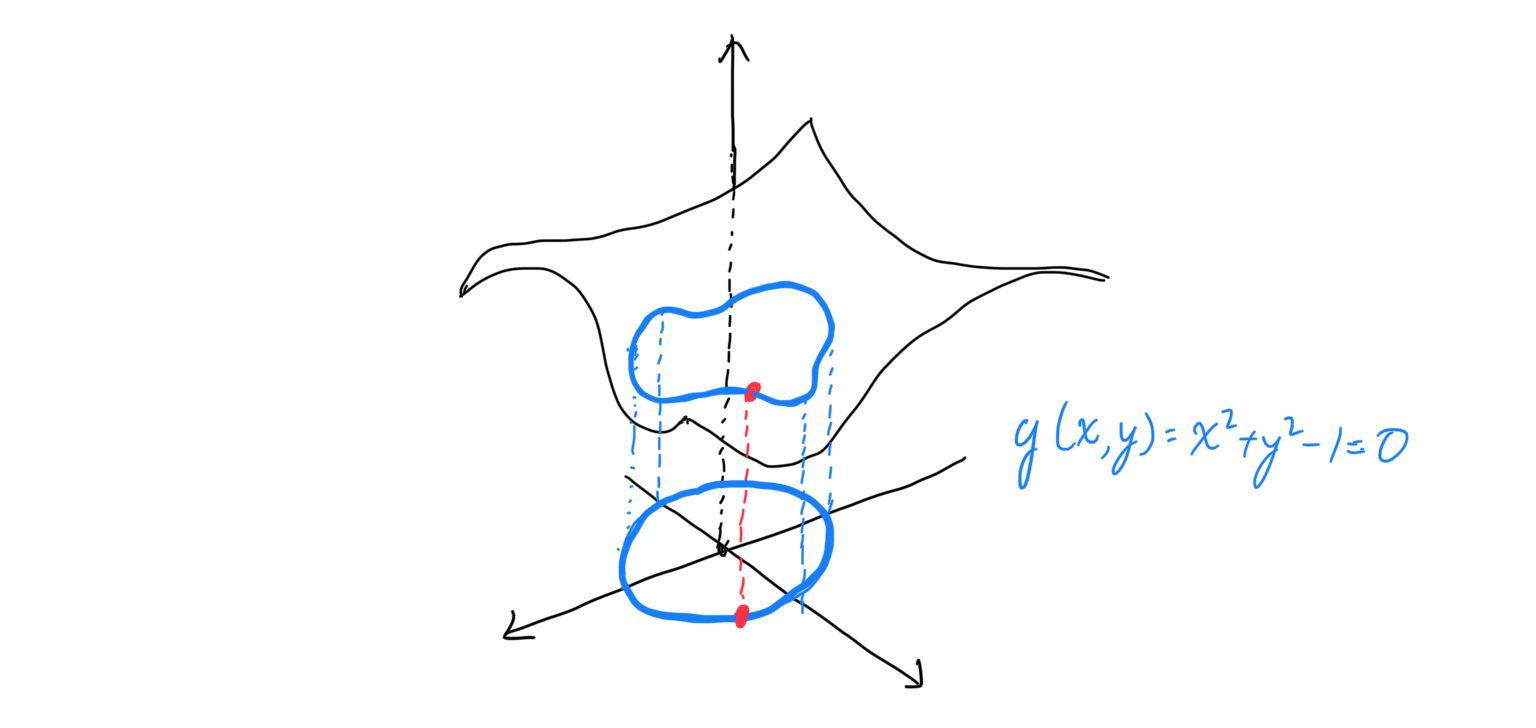
\includegraphics[scale=0.2]{img/Function_with_Constraints.PNG}
  \end{center}
  To solve this constraint problem, we use the method of Lagrange multipliers. The basic idea is to convert a constrained problem into a form such that the derivative test of an unconstrained problem can still be applied. The relationship between the gradient of the function and gradients of the constraints rather naturally leads to a reformulation of the original problem, known as the \textit{Lagrangian function}. That is, in order to find the maximum/minimum of $f$ subjected to the equality constraint $\mathbf{g}(\mathbf{x}) = \mathbf{0}$, we form the Lagrangian function
  \[\mathcal{L}(\mathbf{x}, \lambda) \equiv f(\mathbf{x}) - \boldsymbol{\lambda}^T \mathbf{g}(\mathbf{x})\]
  and find the stationary points of $\mathcal{L}$ considered as a function of $\mathbf{x} \in D$ and the Lagrange multiplier $\lambda \in \mathbb{R}$. The main advantage to this method is that it allows the optimization to be solved without explicit parameterization in terms of the constraints. 

  \begin{theorem}[Lagrange Multipliers Theorem]
  Let $f: \mathbb{R}^n \longrightarrow \mathbb{R}$ be a $C^1$ function and let $g(\mathbf{x}) = 0$, where $g: \mathbb{R}^n \longrightarrow \mathbb{R}^c$, be a system of $C^1$ constraint equations: $g \coloneqq (g_1, g_2, \ldots, g_c)$. Let $\mathbf{x}^*$ be an optimal solution to the optimization problem of maximizing $f(\mathbf{x})$ subject to the constraint $g(\mathbf{x}) = 0$ such that $\rank D g_{\mathbf{x}^*} = c < n$. Then, their exists a unique vector $\boldsymbol{\lambda}^*$ of Lagrange multipliers $\lambda_1^*, \lambda_2^*, \ldots, \lambda_c^*$ s.t. 
  \[D f_{\mathbf{x}^*} = \lambda^{*T} D g_{\mathbf{x}^*}\]
  where $D f_{\mathbf{x}^*}$ can be interpreted as the $1 \times n$ Jacobian matrix of $f$ and $D g_{\mathbf{x}^*}$ as the $c \times n$ Jacobian of $g$. Since both $D f_{\mathbf{x}^*}$ and $\lambda^{*T} D g_{\mathbf{x}^*}$ are maps from $\mathbb{R}^n$ to $\mathbb{R}$, we can invoke Riesz representation theorem to turn this into gradients: 
  \[\nabla f(\mathbf{x}^*) = \nabla \mathbf{g}(\mathbf{x}^*) (\boldsymbol{\lambda}^*)\]
  which has a matrix realization of 
  \begin{align*}
  \begin{pmatrix}
  \frac{\partial f}{\partial x_1} (\mathbf{x}^*) \\ \vdots\\ \frac{\partial f}{\partial x_n} (\mathbf{x}^*) \end{pmatrix} & = \begin{pmatrix}
  \frac{\partial g_1}{\partial x_1} (\mathbf{x}^*)& \ldots & \frac{\partial g_c}{\partial x_1} (\mathbf{x}^*)\\
  \vdots & \ddots & \vdots \\
  \frac{\partial g_1}{\partial x_n} (\mathbf{x}^*)& \ldots & \frac{\partial g_c}{\partial x_n}(\mathbf{x}^*)
  \end{pmatrix} \begin{pmatrix}
  \lambda^*_1 \\ \vdots \\ \lambda^*_c \end{pmatrix} \\
  & = \lambda^*_1 \begin{pmatrix}
  \frac{\partial g_1}{\partial x_1} (\mathbf{x}^*) \\ \vdots \\ \frac{\partial g_1}{\partial x_n}(\mathbf{x}^*)
  \end{pmatrix} + \lambda^*_2 \begin{pmatrix}
  \frac{\partial g_2}{\partial x_1} (\mathbf{x}^*) \\ \vdots \\ \frac{\partial g_2}{\partial x_n}(\mathbf{x}^*)
  \end{pmatrix} + \ldots + \lambda^*_c \begin{pmatrix}
  \frac{\partial g_c}{\partial x_1} (\mathbf{x}^*) \\ \vdots \\ \frac{\partial g_c}{\partial x_n}(\mathbf{x}^*)
  \end{pmatrix}
  \end{align*}
  This equation tells us that at any critical points $\mathbf{x}^*$ of $f$ evaluated under the equality constraints, the gradient of $f$ at $\mathbf{x}^*$ can be expressed as a unique linear combination of the gradients of the constraints $\nabla g_i (\mathbf{x}^*)$ (at $\mathbf{x}^*$), with the Lagrange multipliers acting as coefficients. Therefore, finding the critical points $\mathbf{x}^*$ of $f$ constrained with $g$ is equivalent to solving the system of $c + n$ equations for the $n$ unknowns in $\mathbf{x}$ and $c$ unknowns in $\boldsymbol{\lambda}$: 
  \begin{align*}
      \mathbf{g}(\mathbf{x}) & = 0 \\ 
      \nabla f(\mathbf{x}) & = \nabla \mathbf{g}(\mathbf{x}) (\boldsymbol{\lambda})
  \end{align*} 
  which can be rewritten as
  \begin{align*}
      c \text{ constraint equations} & \begin{cases}
      g_1 (x) & = 0 \\
      \ldots & = 0 \\
      g_c (x) & = 0
      \end{cases} \\
      n \text{ Lagranaian equations} & \begin{cases}
     \frac{\partial f}{\partial x_1} (\mathbf{x}^*) & = \lambda^*_1 \frac{\partial g_1}{\partial x_1} (\mathbf{x}^*) + \lambda^*_2 \frac{\partial g_2}{\partial x_1} (\mathbf{x}^*) + \ldots + \lambda^*_c \frac{\partial g_c}{\partial x_1} (\mathbf{x}^*) \\
      \ldots & = \ldots \\
      \frac{\partial f}{\partial x_n} (\mathbf{x}^*) & = \lambda^*_1 \frac{\partial g_1}{\partial x_n} (\mathbf{x}^*) + \lambda^*_2 \frac{\partial g_2}{\partial x_n} (\mathbf{x}^*) + \ldots + \lambda^*_c \frac{\partial g_c}{\partial x_n} (\mathbf{x}^*) 
      \end{cases}
  \end{align*}
  \end{theorem}

  More abstractly, $D f_{\mathbf{x}^*}$ is the linear functional in $(\mathbb{R}^n)^*$, and $D g_{\mathbf{x}^*}$, which is a linear map from $\mathbb{R}^n$ to $\mathbb{R}^c$, can be interpreted as a map from $(\mathbb{R}^c)^*$ to $(\mathbb{R}^n)^*$ Since $\boldsymbol{\lambda}^*$ "lives" in $(\mathbb{R}^c)^*$, $D g_{\mathbf{x}^*}(\boldsymbol{\lambda}^*) \in (\mathbb{R}^n)^*$, which is the same space that $f_{\mathbf{x}^*}$ lives in. 


  Let us introduce a visualization for when where is a single constraint $g: \mathbb{R}^n \longrightarrow \mathbb{R}$. From the properties of the gradient, $\nabla f(x_0)$ is orthogonal to the level set of points satisfying $f(x) = f(x_0)$ at point $x_0$. Note that the constraint function $g$ also maps $\mathbb{R}^n \longrightarrow \mathbb{R}$, and so it has its own level surfaces. We can see that the point where the contour line of $g(x) = 0$ tangentially touches the contours of $f$ is the maximum. Since it intersects it tangentially, the gradient vector at that point $\nabla g(x_0)$ is parallel to $\nabla f(x_0)$. 
  \begin{center}
      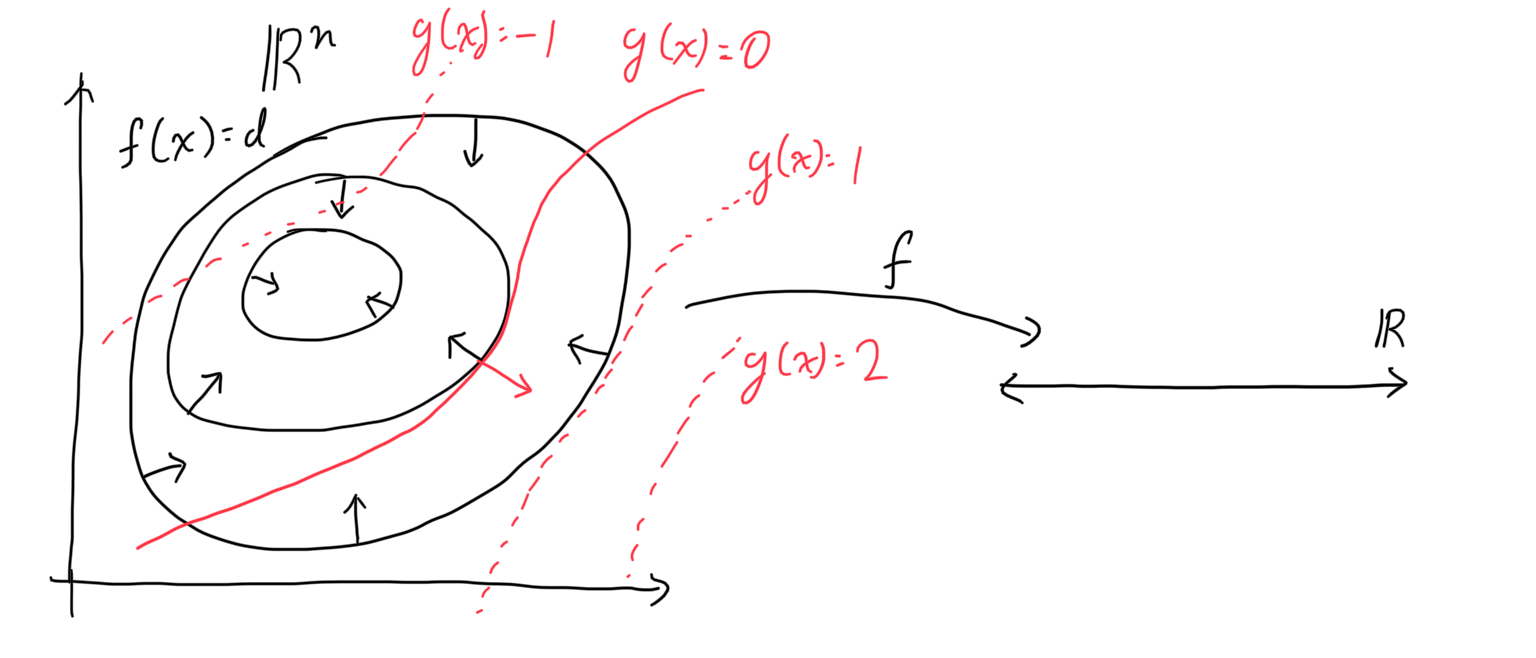
\includegraphics[scale=0.22]{img/Lagrange_Multiplier_Single_Constraint.PNG}
  \end{center}
  We can visualize this for multiple constraints as well, where $\nabla f(x_0)$ (the gradient vector of $f$ at $x^*$) can be expressed as a linear combination of $\nabla g_1 (x_0)$ and $\nabla g_2 (x_0)$ (gradient vectors of the constraint functions at $x^*$). 
  \begin{center}
      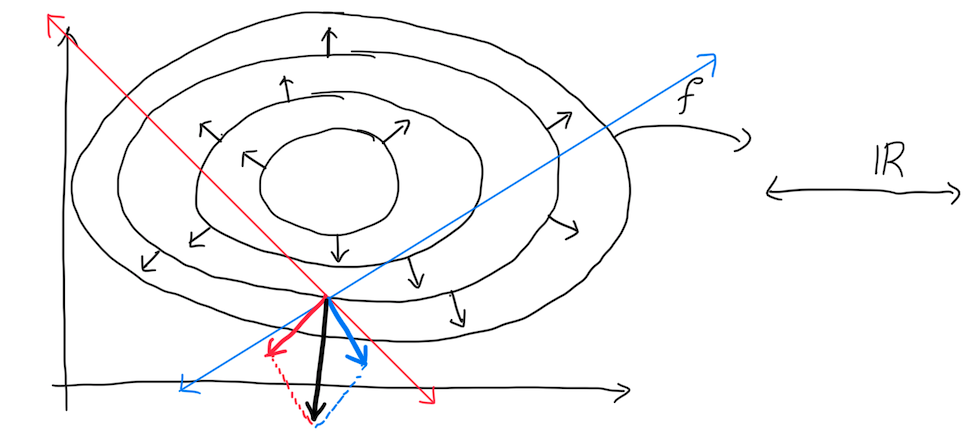
\includegraphics[scale=0.27]{img/Lagrange_Multiplier_Multiple_Constraints.PNG}
  \end{center}

  From the properties of the gradient introduced before, $\triangledown f(x_0)$ is orthogonal to the level set of points satisfying $f(x) = c$ at the point $x_0$. But this level set $f(x) = c$ actually intersects the level set determined by $g(x) = c$ at the point $x_0$ and is indistinguishable from each other at $x_0$. This means that $\triangledown g(x_0)$ is normal the level set of $g(x) = c$ at $x_0 \iff $ it is normal to the level set of $f(x) = c$ at $x_0$. But $\triangledown f(x_0)$ is also normal at that point, so $\triangledown f(x_0)$ must be parallel to $\triangledown g(x_0)$. 
 
\subsection{Inverse and Implicit Function Theorems} 

  \begin{theorem}[Inverse Function Theorem for Multivariable Functions and its Matrix Realization]
  Let $\mathbf{f}: \mathbb{R}^n \longrightarrow \mathbb{R}^n$ be a $C^1$ function defined on an open neighborhood of $\mathbf{x}_0$ in the domain. If the total derivative/Jacobian $D \mathbf{f}_{\mathbf{x}_0}$ at $\mathbf{x}_0$ is invertible, an inverse function of $\mathbf{f}$ is defined on some neighborhood of $\mathbf{y}_0 = \mathbf{f}(\mathbf{x}_0)$. Given that we are working with a fixed basis, $\mathbf{f}$ can be modeled by the set of $n$ equations 
  \begin{align*}
      f_1 (x_1, x_2, \ldots, x_n) &= y_1 \\
      \ldots & = \ldots \\
      f_2 (x_1, x_2, \ldots, x_n) &= y_2
  \end{align*}
  This theorem says that this system of $n$ equations has a unique solution for $x_1, x_2, \ldots, x_n$ in terms of $y_1, \ldots, y_n$, provided that we restrict $\mathbf{x}$ and $\mathbf{y}$ to small enough neighborhoods of $\mathbf{x}_0$ and $\mathbf{y}_0$. This inverse function $\mathbf{f}^{-1}: \mathbb{R}^n \longrightarrow \mathbb{R}^n$ is also $C^1$, and its total derivative/Jacobian $D \mathbf{f}^{-1}_{\mathbf{y}_0}$ at $\mathbf{y}_0 = \mathbf{f}(\mathbf{x}_0)$ is the inverse linear map of $D \mathbf{f}_{\mathbf{y}_0}$. 
  \[D \mathbf{f}^{-1}_{\mathbf{y}_0} = \big( D \mathbf{f}_{\mathbf{x}_0} \big)^{-1}\]
  \end{theorem}

  \begin{example}
  Consider the vector-valued function $\mathbf{f}: \mathbb{R}^2 \longrightarrow \mathbb{R}^2$ defined by 
  \[\mathbf{f}(x_1, x_2) = \begin{pmatrix}
  e^{x_1}\cos (x_2) \\ e^{x_1} \sin(x_2)
  \end{pmatrix}\]
  The total derivative/Jacobian matrix is 
  \[J \mathbf{f}(x_1, x_2) = \begin{pmatrix}
  e^{x_1} \cos(x_2) & - e^{x_1} \sin(x_2) \\
  e^{x_1} \sin(x_2) & e^{x_1} \cos(x_2)
  \end{pmatrix} \implies \det J \mathbf{f}(x_1, x_2) = e^{2x_1} \cos^2 (x_2) + e^{2x_1} \sin^2 (x_2) = e^{2x_1}\]
  Since the determinant $e^{2x_1}$ is nonzero everywhere, $D \mathbf{f}_\mathbf{x}$ is nonsingular. Thus, the theorem guarantees that for every point $\mathbf{x}_0 \in \mathbb{R}^2$, there exists a neighborhood about $\mathbf{x}_0$ over which $\mathbf{f}$ is invertible. However, this does not mean $\mathbf{f}$ is invertible over its entire domain: in this case $\mathbf{f}$ isn't even injective since it is periodic: e.g. the preimage of $(e, 0)$ contains $(1, 0)$ and $(1, 2\pi)$. 
  \end{example}

  Remember that given an explicit representation of a set $\mathbf{y} = \mathbf{f}(\mathbf{x})$, we can easily find the implicit form as $\mathbf{F}(\mathbf{x}, \mathbf{y}) = \mathbf{y} - \mathbf{f}(\mathbf{x}) = \mathbf{0}$. What about the other way around? That is, given an implicit representation of some surface, what conditions must be met so that it can be represented as the graph of a function? The implicit function theorem is a tool that allows relations between points in $\mathbb{R}^n$ to be converted to functions of several real variables. That is, it states that for sufficiently "nice" points on a $n$-dimensional surface defined as $\mathbf{F}(\mathbf{x}, \mathbf{y}) = \mathbf{0}$ (where $\mathbf{F}: \mathbb{R}^{n+m} \longrightarrow \mathbb{R}^m$), we can locally pretend that this surface is a graph of a function $\mathbf{g}: \mathbb{R}^n \longrightarrow \mathbb{R}^m$ whose graph $\big(\mathbf{x}, \mathbf{g}(\mathbf{x})\big)$ is precisely the set of all $(\mathbf{x}, \mathbf{y})$ s.t. $\mathbf{f}(\mathbf{x}, \mathbf{y}) = \mathbf{0}$. When $m = 1$, it basically states that if an implicit surface suffices the vertical line test in a neighborhood, then it can be written as a function. 

  \begin{example}[Circle]
    Let $f: \mathbb{R}^2 \longrightarrow \mathbb{R}$ be defined by $f(x, y) = x^2 + y^2 - 1$. The level set at $z = 0$ would be the set of points satisfying 
    \[x^2 + y^2 - 1 = 0\]
    the unit circle. The derivative of $f$ with respect to $y$ is $0$ at the points $(-1,0)$ and $(1,0)$, meaning that in any neighborhood of these points, we cannot define a function of $y$ with respect to $x$. This is true, indeed, since any such function would fail the vertical line test, which can be seen in the red neighborhood around $(1,0)$. However, the blue neighborhood of the point $(-\sqrt{2}/2, \sqrt{2}/2)$ does indeed define a function of $y$ with respect to $x$ satisfying the vertical line test. 
    \begin{center}
    \begin{tikzpicture}
      \draw[<->] (-3,0)--(3,0);
      \draw[<->] (0,-3)--(0,3);
      \draw (0,0) circle (2);
      \draw[fill=red] (2,0) circle (0.08);
      \draw[fill=red] (-2,0) circle (0.08);
      \draw[red, thick] (1.732, -1) arc (-30:60:2);
      \draw[dashed, <->] (1.8,-2.5)--(1.8,2.5);
      \draw[fill=blue] (-1.414, 1.414) circle (0.08);
      \draw[blue, thick] (-1, 1.732) arc (120:170:2);
      \draw[dashed,<->] (-1.7,2.5)--(-1.7,-2.5);
    \end{tikzpicture}
    \end{center}
  \end{example}

  \begin{theorem}[Special Implicit Function Theorem]
    Let $f: \mathbb{R}^{n+1} \longrightarrow \mathbb{R}$ be a $C^1$ function with a point $(\mathbf{a}, b) \in \mathbb{R}^{n+1}$ on the level set $f(\mathbf{x}, y) = 0$. If $\partial_y f (\mathbf{a}, b)$, which can also be thought of as the $1 \times 1$ truncated Jacobian matrix $D_\mathbf{y} f_{(\mathbf{a}, b)} = \partial_{y} f(\mathbf{a}, b)$ w.r.t. $y$, of 
    \[D f_{(\mathbf{a}, b)} = \begin{pmatrix} D_\mathbf{x} f_{(\mathbf{a}, b)} & D_\mathbf{y} f_{(\mathbf{a}, b)} \end{pmatrix} = \left(\begin{array}{ccc|c}
       \partial_{x_1} f(\mathbf{a}, b) &\ldots & \partial_{x_n} f(\mathbf{a}, b) & \partial_{y} f(\mathbf{a}, b)
       \end{array}\right)\]
    is invertible (in this case nonzero), then there exists an open neighborhood $U_\mathbf{a} \subset \mathbb{R}^n$ of $\mathbf{a}$ and a unique $C^1$ function $y: U \subset \mathbb{R}^n \longrightarrow \mathbb{R}$ s.t. $f\big(\mathbf{x}, y(\mathbf{x})\big) = 0$ for all $\mathbf{x} \in U$. That is, we can find a $y: U \longrightarrow \mathbb{R}$ s.t. the graph $y(\mathbf{x})$ within $U$ coincides with the graph of $f(\mathbf{x}, y) = 0$. Moreover, the total derivative/Jacobian of $y: \mathbb{R}^n \longrightarrow \mathbb{R}$ in $U$ is the $1 \times n$ matrix given by the matrix product
    \[D g_\mathbf{a} = - (D_y f_\mathbf{a})^{-1} D_\mathbf{x} f_\mathbf{a}\]
  \end{theorem}

  \begin{example}[Circle Example]
    Let $n = m = 1$ and $f(x_1, x_2) = x_1^2 + x_2^2 - 1$. We would like to find out at which points $\mathbf{a}$ can this surface be explicitly represented by a function $g: U_\mathbf{a} \subset \mathbb{R} \longrightarrow \mathbb{R}$ defining $x_2$ from $x_1$. Its Jacobian is 
    \[D f = \begin{pmatrix} \partial_{x_1} f & \partial_{x_2} f \end{pmatrix} = \begin{pmatrix} 2 x_1 & 2x_2 \end{pmatrix} \]
    The truncated Jacobian w.r.t. $x_2$ is $2 x_2$, which is invertible iff $x_2 \neq 0$. By the implicit function theorem, we can locally write the circle in the form $x_2 = g(x_1)$ for all points where $x_2 \neq 0$. This is easy to see. For example, we can choose the point $(0.8, 0.6)$ on the level set, and the appropriate explicit function is 
    \[x_2 = g(x_1) = \sqrt{1 - x_1^2}\]
    within the neighborhood of $x_1 = 0.8$. For $(\pm 1, 0)$, we cannot since every function defined within a neighborhood of $x_1 = \pm 1$ fails the vertical line test. The derivative of $g$, by the theorem, can be defined implicitly as 
    \[D g = - ( \partial_{x_2} f)^{-1} D_{x_1} f = - (2 x_2)^{-1} (2 x_1) = -\frac{x_1}{x_2}\]
    which leads to the differential equation 
    \[g^\prime (x_1) = - \frac{x_1}{g(x_1)} \text{ where we solve for } g\]
    If we would have liked to find a function $h: U_{a_{\mathbf{x}_2}} \subset \mathbb{R} \longrightarrow \mathbb{R}$ defining $x_1$ from $x_2$, then we can redo everything to find that the truncated Jacobian w.r.t. $x_1$ is $2x_1$, which is invertible iff $x_1 \neq 0$, and the the derivative is 
    \[D h = - (\partial_{x_1} f)^{-1} D_{x_2} f = - (2x_1)^{-1} (2x_2) = -\frac{x_2}{x_1}\]
    which leads to the differential equation 
    \[h^\prime (x_2) = - \frac{x_2}{h(x_2)} \text{ where we solve for } h\]
  \end{example}

  \begin{theorem}[General Implicit Function Theorem]
    Let $f: \mathbb{R}^{n+m} \longrightarrow \mathbb{R}^m$ be a $C^1$ function with a point $(\mathbf{a}, \mathbf{b}) \in \mathbb{R}^{n + m}$ on the level set $f( \mathbf{x}, \mathbf{y}) = 0$. If the $m \times m$ truncated Jacobian matrix $D_{\mathbf{y}} f (\mathbf{a}, \mathbf{b})$ w.r.t. $\mathbf{y}$, of 
    \[D f_{(\mathbf{a}, \mathbf{b})} = \begin{pmatrix} D_\mathbf{x} f_{(\mathbf{a}, \mathbf{b})} & D_\mathbf{y} f_{(\mathbf{a}, \mathbf{b})} \end{pmatrix}\]
    is invertible, then there exists an open neighborhood $U_\mathbf{a} \subset \mathbb{R}^n$ of $\mathbf{a}$ and a unique $C^1$ function $\mathbf{y}: U \subset \mathbb{R}^n \longrightarrow \mathbb{R}^m$ s.t. $f\big(\mathbf{x}, \mathbf{y}(\mathbf{x}) \big) = 0$ for all $\mathbf{x} \in U$. That is, we can find a $\mathbf{y}: U \longrightarrow \mathbb{R}^m$ s.t. the graph $\mathbf{y}(\mathbf{x})$ within $U$ coincides with the graph of $f(\mathbf{x}, \mathbf{y}) = 0$. Moreover, the total derivative/Jacobian of $\mathbf{y}$ is the $m \times n$ matrix given by the matrix product 
    \[D g_\mathbf{a} = - (D_\mathbf{y} f_\mathbf{a})^{-1} D_\mathbf{x} f_\mathbf{a}\]
  \end{theorem}

